% !TEX TS-program = XeLaTeX
% use the following command:
% all document files must be coded in UTF-8
\documentclass[spanish]{textolivre}
% build HTML with: make4ht -e build.lua -c textolivre.cfg -x -u article "fn-in,svg,pic-align"
\usepackage{enumitem} % Pacote necessário para controlar o estilo da lista
\usepackage{multirow}

\journalname{Texto Livre}
\thevolume{19}
%\thenumber{1} % old template
\theyear{2026}
\receiveddate{\DTMdisplaydate{2025}{11}{28}{-1}} % YYYY MM DD
\accepteddate{\DTMdisplaydate{2026}{1}{19}{-1}}
\publisheddate{\DTMdisplaydate{2026}{5}{30}{-1}}
\corrauthor{Steffanie Kloss}
\articledoi{10.1590/1983-3652.2026.63123}
%\articleid{NNNN} % if the article ID is not the last 5 numbers of its DOI, provide it using \articleid{} commmand 
% list of available sesscions in the journal: articles, dossier, reports, essays, reviews, interviews, editorial
\articlesessionname{dossier}
\runningauthor{Kloss, Cordovez-Fernández y Bustamante} 
%\editorname{Leonardo Araújo} % old template
\sectioneditorname{Camila Cárdenas Neira~\orcid{0000-0002-1842-7200}}
\layouteditorname{Saula Cecília~\orcid{0009-0006-3069-8480}}

\title{Evaluación de la calidad de escritura en ensayos argumentativos: comparación entre Grandes Modelos de Lenguaje (LLM) y revisiones humanas basadas en una rúbrica}
\othertitle{Avaliação da qualidade da escrita em ensaios argumentativos: comparação entre Modelos Linguísticos Amplos (LLM) e avaliações humanas baseadas em uma rubrica}
% if there is a third language title, add here:
\othertitle{Evaluation of writing quality in argumentative essays: comparison between Large Language Models (LLM) and human reviews based on a rubric}

\author[1]{Steffanie Kloss~\orcid{0000-0001-7018-5395}\thanks{Email: \href{mailto:steffanie.kloss@unab.cl}{steffanie.kloss@unab.cl}}}
\author[2]{Maximiliano Cordovez-Fernández~\orcid{0009-0002-3365-1451}\thanks{Email: \href{mailto:maximiliano.cordovez.f@mail.pucv.cl}{maximiliano.cordovez.f@mail.pucv.cl}}}
\author[3]{Cristóbal Bustamante~\orcid{0009-0003-1563-7901}\thanks{Email: \href{mailto:cristobal.bustamante@pucv.cl}{cristobal.bustamante@pucv.cl}}}
\affil[1]{Universidad Andrés Bello, Facultad de Educación y Humanidades, Santiago, Chile.}
\affil[2]{Pontificia Universidad Católica de Valparaíso, Instituto de Literatura y Ciencias del Lenguaje, Valparaíso, Chile.}
\affil[3]{Pontificia Universidad Católica de Valparaíso, Escuela de Pedagogía, Valparaíso, Chile.}

\addbibresource{article.bib}
% use biber instead of bibtex
% $ biber article

% used to create dummy text for the template file
\definecolor{dark-gray}{gray}{0.35} % color used to display dummy texts
\usepackage{lipsum}
\SetLipsumParListSurrounders{\colorlet{oldcolor}{.}\color{dark-gray}}{\color{oldcolor}}

% used here only to provide the XeLaTeX and BibTeX logos
\usepackage{hologo}

% if you use multirows in a table, include the multirow package
\usepackage{multirow}

% provides sidewaysfigure environment
\usepackage{rotating}

% CUSTOM EPIGRAPH - BEGIN 
%%% https://tex.stackexchange.com/questions/193178/specific-epigraph-style
\usepackage{epigraph}
\renewcommand\textflush{flushright}
\makeatletter
\newlength\epitextskip
\pretocmd{\@epitext}{\em}{}{}
\apptocmd{\@epitext}{\em}{}{}
\patchcmd{\epigraph}{\@epitext{#1}\\}{\@epitext{#1}\\[\epitextskip]}{}{}
\makeatother
\setlength\epigraphrule{0pt}
\setlength\epitextskip{0.5ex}
\setlength\epigraphwidth{.7\textwidth}
% CUSTOM EPIGRAPH - END

% to use IPA symbols in unicode add
%\usepackage{fontspec}
%\newfontfamily\ipafont{CMU Serif}
%\newcommand{\ipa}[1]{{\ipafont #1}}
% and in the text you may use the \ipa{...} command passing the symbols in unicode

% LANGUAGE - BEGIN
% ARABIC
% for languages that use special fonts, you must provide the typeface that will be used
% \setotherlanguage{arabic}
% \newfontfamily\arabicfont[Script=Arabic]{Amiri}
% \newfontfamily\arabicfontsf[Script=Arabic]{Amiri}
% \newfontfamily\arabicfonttt[Script=Arabic]{Amiri}
%
% in the article, to add arabic text use: \textlang{arabic}{ ... }
%
% RUSSIAN
% for russian text we also need to define fonts with support for Cyrillic script
% \usepackage{fontspec}
% \setotherlanguage{russian}
% \newfontfamily\cyrillicfont{Times New Roman}
% \newfontfamily\cyrillicfontsf{Times New Roman}[Script=Cyrillic]
% \newfontfamily\cyrillicfonttt{Times New Roman}[Script=Cyrillic]
%
% in the text use \begin{russian} ... \end{russian}
% LANGUAGE - END

% EMOJIS - BEGIN
% to use emoticons in your manuscript
% https://stackoverflow.com/questions/190145/how-to-insert-emoticons-in-latex/57076064
% using font Symbola, which has full support
% the font may be downloaded at:
% https://dn-works.com/ufas/
% add to preamble:
% \newfontfamily\Symbola{Symbola}
% in the text use:
% {\Symbola }
% EMOJIS - END

% LABEL REFERENCE TO DESCRIPTIVE LIST - BEGIN
% reference itens in a descriptive list using their labels instead of numbers
% insert the code below in the preambule:
%\makeatletter
%\let\orgdescriptionlabel\descriptionlabel
%\renewcommand*{\descriptionlabel}[1]{%
%  \let\orglabel\label
%  \let\label\@gobble
%  \phantomsection
%  \edef\@currentlabel{#1\unskip}%
%  \let\label\orglabel
%  \orgdescriptionlabel{#1}%
%}
%\makeatother
%
% in your document, use as illustraded here:
%\begin{description}
%  \item[first\label{itm1}] this is only an example;
%  % ...  add more items
%\end{description}
% LABEL REFERENCE TO DESCRIPTIVE LIST - END


% add line numbers for submission
%\usepackage{lineno}
%\linenumbers

\begin{document}
\maketitle

\begin{polyabstract}
\begin{abstract}
La evaluación automática de la escritura se ha consolidado como una alternativa prometedora para agilizar y mejorar la retroalimentación en el aprendizaje a causa del desarrollo de la Inteligencia Artificial Generativa (IAG) con los Grandes Modelos de Lenguaje (LLM) como ChatGPT de OpenAI. De este modo, la retroalimentación formativa que proporcionan las IAs tienen el potencial de influir en la autorregulación y la mejora continua del desempeño académico del estudiantado. De acuerdo con este contexto, el objetivo de este trabajo es determinar el grado de fiabilidad interjueces en la evaluación de ensayos argumentativos realizada por modelos de lenguaje (GPTo3-mini-high y GPT-4), comparándola con la evaluación de un experto humano mediante la rúbrica analítica RUBRIAR. Se utilizó un enfoque cuantitativo para determinar el grado de concordancia entre las evaluaciones realizadas por el experto y las realizadas por los modelos ChatGPT personalizados en 46 ensayos argumentativos escritos por estudiantes universitarios de primer año. Los hallazgos revelan que la evaluación efectuada por los LLM es similar a la del humano experto, especialmente en la dimensión de ajuste al género en la subdimensión de propósito comunicativo. Sin embargo, hay una baja precisión en las relaciones de cohesión y coherencia, así como con el ajuste a las normas de la lengua. Se concluye que es fundamental incorporar un enfoque pedagógico que promueva un uso intencionado, reflexivo y ético de herramientas de IA, particularmente durante los primeros años de la educación superior, cuando los estudiantes están construyendo las bases de sus competencias académicas.

\keywords{Evaluación de la escritura\sep Inteligencia Artificial Generativa\sep Ensayo\sep Calidad de la escritura}
\end{abstract}

\begin{portuguese}
\begin{abstract}
A avaliação automatizada da escrita manual consolidou-se como uma alternativa promissora para otimizar e aprimorar o feedback no aprendizado, graças ao desenvolvimento da Inteligência Artificial Generativa (IAG) com Grandes Modelos de Linguagem (MLLs), como o ChatGPT da OpenAI. Dessa forma, o feedback formativo fornecido pelas IAs tem o potencial de influenciar a autorregulação e a melhoria contínua do desempenho acadêmico dos alunos. De acordo com este contexto, o objetivo deste trabalho é determinar o grau de confiabilidade interjuízes na avaliação de ensaios argumentativos realizada por modelos de linguagem (GPTo3-mini-high e GPT-4), comparando-a com a avaliação de um especialista humano por meio da rubrica analítica RUBRIAR. Utilizou-se uma abordagem quantitativa para determinar o grau de concordância entre as avaliações realizadas pelo especialista e as realizadas pelos modelos ChatGPT personalizados em 46 ensaios argumentativos escritos por estudantes universitários do primeiro ano. Os resultados revelam que a avaliação feita pelos LLM é semelhante à do especialista humano, especialmente na dimensão de ajuste ao gênero na subdimensão de propósito comunicativo. No entanto, há uma baixa precisão nas relações de coesão e coerência, bem como no ajuste às normas da língua. Conclui-se que é essencial incorporar uma abordagem pedagógica que promova o uso intencional, reflexivo e ético das ferramentas de IA, particularmente durante os primeiros anos do ensino superior, quando os alunos estão construindo as bases de suas competências acadêmicas.

\keywords{Avaliação da escrita\sep Inteligência Artificial Generativa\sep Ensaio\sep Qualidade da escrita}
\end{abstract}
\end{portuguese}
% if there is another abstract, insert it here using the same scheme

\begin{english}
\begin{abstract}
Automated handwriting assessment has established itself as a promising alternative to streamline and improve feedback in learning due to the development of Generative Artificial Intelligence (GAI) with Large Language Models (LLMs) such as OpenAI's ChatGPT. Thus, the formative feedback provided by AI has the potential to influence self-regulation and continuous improvement in student academic performance. In this context, the objective of this study is to determine the degree of inter-rater reliability in the evaluation of argumentative essays performed by language models (GPTo3-mini-high and GPT-4), comparing it with the evaluation of a human expert using the RUBRIAR analytical rubric. A quantitative approach was used to determine the degree of agreement between the evaluations made by the expert and those made by the customized ChatGPT models on 46 argumentative essays written by first-year university students. The findings reveal that the evaluation performed by the LLMs is similar to that of the human expert, especially in the dimension of gender adjustment in the subdimension of communicative purpose. However, there is low accuracy in cohesion and coherence relationships, as well as in conformity with language norms. It is concluded that it is essential to incorporate a pedagogical approach that promotes an intentional, reflective, and ethical use of AI tools, particularly during the early years of higher education, when students are building the foundations of their academic competencies.

\keywords{Writing assessment\sep Generative Artificial Intelligence\sep Essay\sep Writing quality}
\end{abstract}
\end{english}
\end{polyabstract}

\section{Introducción}
Evaluar la escritura constituye una de las tareas más complejas y demandantes dentro del proceso de enseñanza porque compromete analizar, juzgar y emitir valoraciones fundamentadas sobre la calidad textual de los escritos del estudiantado \cite{prado2021}. Esta tarea no solo exige la evaluación y corrección de errores, sino que implica una comprensión profunda de los procesos cognitivos, discursivos y lingüísticos relacionados con la producción escrita \cite{hayes2012}. En el contexto universitario, la evaluación adquiere un nivel adicional de complejidad, tanto por el elevado volumen de textos que deben revisarse como por la necesidad de aplicar criterios que garanticen equidad, validez y fiabilidad en los juicios emitidos \cite{carless2020, tardy2020}. De este modo, la evaluación escrita cumple una doble función: por un lado, tiene un carácter certificador, al determinar el nivel de logro alcanzado; y, por otro, un carácter formativo, pues promueve la autorregulación y la conciencia metacognitiva al permitir la reflexión sobre el propio desempeño \cite{kloss-tapia2025, kloss2023, castello2011}. 

Aunque el ámbito educativo demanda respuestas cada vez más individualizadas y personalizadas, los recursos de tiempo y personal siguen siendo limitados \cite{sologuren2023}. En este escenario, el reciente auge de los modelos de lenguaje basados en inteligencia artificial (IA) ha generado un terreno fértil para la innovación pedagógica \cite{unesco2024}. En particular, los avances en modelos de lenguaje de gran escala (LLM) ofrecen nuevas posibilidades para analizar y valorar textos escritos con niveles de coherencia y pertinencia sofisticados. Las denominadas IA generativas se distinguen por su capacidad para producir, sintetizar, reformular y evaluar información de manera autónoma, posicionándose como potenciales aliados en los procesos de revisión y evaluación de la escritura académica \cite{poole2024}.

En la última década, los modelos de lenguaje basados en IA no solo se han expandido con rapidez, sino que han comenzado a transformar prácticas concretas, entre ellas la evaluación y la retroalimentación de la escritura. Su incorporación en estos procesos ha abierto nuevas vías metodológicas como el análisis inmediato, la personalización de comentarios y el apoyo al desarrollo de competencias escritas, lo que explica el interés que han despertado en la comunidad científica \cite{ossa2023, poole2024, teng-ma2024, teng2025, garciafernandez2025}.

Durante la última década, la expansión de los LLM ha transformado múltiples ámbitos de la vida social y profesional. En este sentido, el campo educativo no ha sido una excepción \cite{mateogirona2025}. Numerosas investigaciones han explorado su potencial en la enseñanza de la escritura, particularmente en la automatización de tareas tradicionalmente manuales, como la retroalimentación escrita \cite{teng2025, poole2024, ossa2023, venegas2022}. En la enseñanza de segundas lenguas, por ejemplo, el enfoque Automated Writing Evaluation (AWE) ha integrado sistemas de IA en procesos de valoración y feedback, con el propósito de ofrecer comentarios inmediatos y personalizados \cite{teng2024, teng2025}. Estos avances han demostrado que la tecnología puede ampliar las oportunidades de práctica y apoyo, al mismo tiempo que reduce la carga docente asociada a la revisión.

Si bien la investigación desarrollada en este ámbito ha aumentado, la mayoría de los estudios se ha concentrado en la retroalimentación formativa, mientras que el uso de la IA en la evaluación propiamente dicha ha recibido menor atención. En otras palabras, el proceso de juzgar la calidad del texto conforme a criterios explícitos y estandarizados aún carece de investigación empírica lo suficientemente robusta.

Persisten, por tanto, interrogantes acerca de la precisión, consistencia y legitimidad de las evaluaciones automatizadas frente a las emitidas por expertos humanos, sobre todo en géneros académicos como el ensayo argumentativo. Investigar sobre el ensayo es un nicho que merece la pena cubrir porque es uno de los más demandados en educación superior \cite{kloss2024} y por sus características, entre las que destaca su organización retórica, la riqueza de su argumentación, la brevedad y la interpretación apoyada en el uso de fuentes teóricas adecuadas \cite{zunino2012}. Además, ofrece a los estudiantes la oportunidad de identificar un problema, adoptar una postura y desarrollarla desde una perspectiva crítica y reflexiva \cite{kloss-burdiles2025}, lo que refuerza la necesidad de comprender cómo los sistemas automatizados evalúan su calidad.

El presente estudio tiene por objetivo determinar el grado de fiabilidad interjueces en la evaluación de ensayos argumentativos realizada por modelos de lenguaje (GPTo3-mini-high y GPT-4), comparándola con la evaluación de un experto humano mediante la rúbrica analítica RUBRIAR \cite{kloss2024} como instrumento de referencia. Se adoptó un enfoque cuantitativo orientado a identificar el grado de concordancia entre la evaluación realizada por expertos y aquellas generadas por dos modelos: (a) un GPT personalizado (GPT-4) y (b) el modelo GPT-o3-mini-high, un modelo razonador que emplea mayor tiempo de cómputo antes de emitir su respuesta; ambos configurados mediante \textit{prompt engineering} para incorporar instrucciones y conocimientos específicos sobre la evaluación. El análisis se efectuó sobre un corpus de 46 ensayos argumentativos producidos por estudiantes de primer año de universidad.


\section{Metodología}
El estudio se enmarca en un enfoque cuantitativo, de carácter comparativo y correlacional, que permitió medir el grado de concordancia entre modelos de lenguaje generativos y un evaluador humano. 

\subsection{Corpus}
El corpus estuvo compuesto por 46 ensayos argumentativos redactados por estudiantes de primer año de una universidad chilena del ámbito de las Ciencias Sociales. La extensión de cada texto tuvo un promedio de 2500 palabras, por lo que el corpus total se constituyó por 115 000 palabras.

\subsection{Instrumentos}
Se aplicó la rúbrica analítica RUBRIAR \cite{kloss2024}. Esta se organiza mediante cuatro dimensiones: ajuste al género discursivo del ensayo, organización retórica del ensayo académico, relaciones de cohesión y coherencia, y ajuste a las normas de la lengua. Además, se consideraron diecisiete subdimensiones, las que en su conjunto permitieron valorar la calidad de los ensayos argumentativos (ver Tabla \ref{tab-1}). Cabe destacar que tanto el experto humano como los modelos de lenguaje aplicaron la rúbrica revisando sistemáticamente cada subdimensión de manera independiente por cada uno de los 46 ensayos revisados, asignando puntajes en una escala de 0 a 5. La evaluación realizada por el experto humano fue auditada por el equipo de investigación, quienes mediante la revisión exhaustiva de cada indicador con el texto y el puntaje asignado, lograron un nivel de acuerdo casi perfecto (k=.81). En cuanto a la evaluación realizada por los modelos de lenguaje, esta se realizó mediante un prompt (ver Anexo \ref{anexo-1}).

%--- inserir tabela 1 ---%
% Tabela 1
\begin{table}[h!]
\centering
\begin{threeparttable}
\caption{Rúbrica analítica RUBRIAR.}\label{tab-1}
\begin{tabular}{p{3.5cm} p{7.2cm} p{2.5cm}}
\toprule
Dimensiones & Subdimensiones & Puntaje total por dimensión \\
\midrule
1. Ajuste al género discursivo del ensayo & Propósito comunicativo; voces del discurso; anidación de la cita; modo de organización del discurso. & 20 puntos \\

2. Organización retórica del ensayo académico & Título; introducción; tesis; argumentación; incorporación de respaldos; condiciones de refutación; conclusión; referencias bibliográficas. & 40 puntos \\

3. Relaciones de cohesión y coherencia & Puntuación y elementos de conexión; progresión y recurrencia; precisión léxica. & 15 puntos \\

4. Ajuste a las normas de la lengua & Ortografía literal; ortografía acentual. & 10 puntos \\
\bottomrule
\end{tabular}
\source{\textcite{kloss2024}.}
\end{threeparttable}
\end{table}

\subsection{Procedimiento}
Para la realización del estudio, se adoptaron ciertas consideraciones técnicas vinculadas al uso de los GPTs. En este caso, se optó por llevar a cabo el análisis de manera manual con el propósito de mantener la interacción lo más cercana posible a una experiencia de uso natural. Esta decisión también respondió al interés de obtener resultados representativos de los modelos, considerando cómo respondería en un contexto de interacción directa y específica con cada usuario. Aunque habría sido posible automatizar el proceso mediante el empleo de la API o el uso de la interfaz de programación, se decidió utilizar la plataforma web de ChatGPT, ingresando y procesando cada texto individualmente. Esta decisión metodológica permitió observar con mayor fidelidad la interacción entre usuario y sistema para garantizar la autenticidad de las respuestas generadas y la validez ecológica del estudio.

Para esta investigación, se utilizó la herramienta de GPT Personalizado (GPT-4) que permite la combinación de instrucciones y conocimientos adicionales y GPT-o3-mini-high. Para la construcción del \textit{prompt} se siguió la técnica de \textit{Prompt engineering} específica de OpenAI que sugiere entregar a ChatGPT un procedimiento paso a paso. Para la creación del prompt, primero se le asignó un rol al modelo, en este caso el de un asistente académico especializado en analizar y calificar ensayos argumentativos de estudiantes universitarios del ámbito de Ciencias Sociales. Segundo, se le solicitó al modelo ejecutar una tarea específica: realizar la revisión de los ensayos mediante la rúbrica RUBRIAR \cite{kloss2024}, la que se compone de cuatro dimensiones y de diecisiete subdimensiones. Cabe destacar que cada una de estas dimensiones y subdimensiones fueron desglosadas dentro del \textit{prompt}, con el fin de facilitar la comprensión y aplicación de los criterios de evaluación por parte de la IA. Además, se le indicó a los modelos de lenguaje que asignaran un puntaje en una escala de 0 a 5 por subdimensión, explicitando dentro del prompt el significado de cada valor de la escala (0, 1, 2, 3, 4 y 5), donde 0 corresponde a una subdimensión ausente en el texto y 5 un desempeño destacado. Tercero, se presentaron las instrucciones para seguir en el análisis, tales como: leer detalladamente cada ensayo, evaluar con máximo rigor cada subdimensión o consultar modelos de referencia proporcionados para la revisión. Cuarto, se presentó la escala de evaluación por cada subdimensión. Quinto, se le solicitó generar una retroalimentación que destaque aspectos positivos y por mejorar para cada subdimensión. De carácter opcional, se especificaron las instrucciones para la generación de un archivo en Excel con la revisión. Posteriormente, se entregaron algunas orientaciones para una evaluación justa siguiendo lineamientos para las calificaciones críticas, es decir, que se evalúe lo que se plantea medir sin subsidiar áreas deficitarias, y, finalmente, se le proporcionó un ejemplo de interacción con la salida esperada (Ver Anexo \ref{anexo-1}).

Es importante señalar que el diseño del \textit{prompt} incorporó principios de \textit{prompt engineering} y se adaptó a las necesidades específicas del \textit{chatbot} con el fin de obtener resultados con mayor precisión. Para ello se realizó una revisión basada en quince ensayos argumentativos, lo que permitió evaluar el \textit{prompt} original y verificar su claridad, coherencia, especificidad y eficacia para producir la respuesta esperada por el modelo. Tras este análisis, el \textit{prompt} fue ajustado y optimizado con el objetivo de mejorar la calidad, precisión y relevancia de las revisiones, desde la contextualización hasta un refinamiento estructural y lingüístico.

\subsection{Análisis de datos}
Una vez realizadas las correcciones por parte del evaluador experto y auditados por el equipo de investigación, los puntajes asignados fueron ingresados a una base de datos para el análisis estadístico, en la que se agrupó la puntuación por dimensión y también de manera global. Este procedimiento se repitió con los dos evaluadores automáticos. En relación con los análisis estadísticos, estos fueron realizados con los software JAMOVI 2.3.28 y JASP; este último utiliza el entorno estadístico de R.

Se procedió con la siguiente estructura de análisis: en primer lugar, se levantaron análisis de estadística descriptiva, para cada dimensión y corrector, incluyendo las medias, desviación estándar, varianza y normalidad de los datos mediante la prueba de Shapiro-Wilk \cite{razali2011}.

En segundo lugar, se evaluó la fiabilidad general entre los tres correctores, mediante el análisis del Coeficiente de Correlación Intraclase (ICC) \cite{shrout1979, koo2016}, proceso replicado para los resultados de cada dimensión de la rúbrica. Se seleccionó el modelo de efectos aleatorios bidireccional para el acuerdo promedio (ICC2k), ya que se busca evaluar la intercambiabilidad de las puntuaciones de los tres correctores. Para complementar el análisis de fiabilidad y examinar el acuerdo entre correctores, se empleó el análisis de Bland-Altman \cite{giavarina2015} con el propósito de determinar el sesgo sistemático y los límites de acuerdo.

Finalmente, para evaluar el efecto del corrector en las dimensiones de las puntuaciones asignadas, se realizó un ANOVA de medidas repetidas. Este análisis incluyó al factor ``corrector'' y al factor ``dimensiones'', al considerar que cada aspecto de la rúbrica fue evaluado de manera repetida por tres correctores.  Para realizar el análisis se verificaron los supuestos de esfericidad mediante la prueba de Mauchly y corrección de grados de libertad de Greenhouse-geisser. Por otro lado, se aplicaron comparaciones \textit{post hoc} para identificar las diferencias específicas.

\section{Resultados}
Las puntuaciones otorgadas por cada evaluador a los ensayos corregidos (N=46) fueron desagregadas en variables independientes según cada dimensión de la rúbrica analítica utilizada en el estudio. En consecuencia, se consideraron los puntajes correspondientes a: (a) Ajuste al género discursivo ensayo (dimensión 1), (b) Organización retórica del ensayo académico (dimensión 2), (c) Relaciones de cohesión y coherencia (dimensión 3) y (d) Ajuste a las normas de la lengua (dimensión 4), así como la puntuación global asignada a cada texto por cada tipo de evaluador.

La Tabla \ref{tab-2} presenta los estadísticos descriptivos de dichas puntuaciones en función del tipo de evaluador (agentes de Inteligencia Artificial y experto humano), incluyendo el tamaño muestral (N=46), la media, la desviación estándar y la varianza. Asimismo, se incorporan los resultados de la prueba de normalidad de Shapiro-Wilk (estadístico $W$ y valor $p$) con el objetivo de evaluar el cumplimiento del supuesto de normalidad de las distribuciones, requisito relevante para la selección de pruebas inferenciales posteriores (ver Tabla \ref{tab-2}).

El análisis descriptivo permitió observar, por una parte, tendencias centrales y niveles de dispersión de las puntuaciones asignadas por cada evaluador en cada dimensión de la rúbrica y, por otra, identificar diferencias en la forma de las distribuciones entre evaluadores y dimensiones. En particular, los resultados de la prueba de Shapiro-Wilk evidencian que la normalidad no se cumple de manera consistente en todas las dimensiones ni para todos los evaluadores, especialmente en las dimensiones asociadas a aspectos de relaciones de cohesión y coherencia, y aspectos normativos (dimensiones 3 y 4), lo que sugiere cierta cautela en la aplicación de pruebas paramétricas y justifica la consideración de procedimientos estadísticos no paramétricos en los análisis comparativos posteriores.

Respecto a los puntajes de cada dimensión, es importante considerar que para cada una los rangos van entre 0 y 5 puntos. La dimensión 1 (Ajuste al género discursivo ensayo) tiene una puntuación máxima de 20 puntos, por lo que las medias de los tres evaluadores fluctúan entre 12,93 y 13,24 puntos. Para la dimensión 2 (Organización retórica del ensayo académico), la puntuación máxima es de 40 puntos, por su parte las medias de los evaluadores se sitúan entre los 24,72 y 25,78. En la dimensión 3 (Relaciones de cohesión y coherencia), el puntaje máximo de la rúbrica es de 15 puntos, cuyas medias establecidas por los evaluadores fluctúan entre los 6,89 y 9,74 puntos. Finalmente, la dimensión 4 (Ajuste a las normas de la lengua), cuenta con una puntuación máxima de 10 puntos, a lo que las medias de los expertos se sitúan entre 6,87 y 7,26.

%--- codigo da tabela 2 ---%
% Tabela 2
\begin{table}[h!]
\centering
\begin{threeparttable}
\caption{Estadística descriptiva de la evaluación de agentes de Inteligencia Artificial y experto humano, por dimensión de la rúbrica.}\label{tab-2}
\small
\begin{tabular}{p{3cm} p{2.5cm} c c c c c c c}
\toprule
Variable & Evaluador & N & Media & \shortstack{Desviación \\ estándar} & Varianza & $W$ & $p$ \\
\midrule
Puntaje Dimensión 1 & GPTo3-mini-high & 46 & 13,24 & 2,04 & 4,14 & 0,934 & 0,012 \\
Puntaje Dimensión 1 & GPT-4 & 46 & 12,98 & 2,39 & 5,71 & 0,919 & 0,003 \\
Puntaje Dimensión 1 & Experto & 46 & 12,93 & 3,12 & 9,75 & 0,958 & 0,094 \\

Puntaje Dimensión 2 & GPTo3-mini-high & 46 & 24,72 & 3,66 & 13,41 & 0,964 & 0,158 \\
Puntaje Dimensión 2 & GPT-4 & 46 & 25,78 & 4,60 & 21,20 & 0,971 & 0,293 \\
Puntaje Dimensión 2 & Experto & 46 & 24,72 & 6,00 & 36,03 & 0,973 & 0,348 \\

Puntaje Dimensión 3 & GPTo3-mini-high & 46 & 9,74 & 1,65 & 2,73 & 0,876 & <,001 \\
Puntaje Dimensión 3 & GPT-4 & 46 & 8,80 & 1,88 & 3,54 & 0,961 & 0,126 \\
Puntaje Dimensión 3 & Experto & 46 & 6,89 & 2,36 & 5,57 & 0,938 & 0,017 \\

Puntaje Dimensión 4 & GPTo3-mini-high & 46 & 7,26 & 1,74 & 3,04 & 0,902 & <,001 \\
Puntaje Dimensión 4 & GPT-4 & 46 & 6,96 & 1,76 & 3,11 & 0,911 & 0,002 \\
Puntaje Dimensión 4 & Experto & 46 & 6,87 & 2,87 & 8,25 & 0,895 & <,001 \\

Puntaje Global & GPTo3-mini-high & 46 & 54,96 & 7,55 & 56,98 & 0,983 & 0,720 \\
Puntaje Global & GPT-4 & 46 & 54,54 & 9,76 & 95,28 & 0,980 & 0,616 \\
Puntaje Global & Experto & 46 & 52,50 & 10,65 & 113,36 & 0,984 & 0,787 \\
\bottomrule
\end{tabular}
\source{Elaboración propia.}
\end{threeparttable}
\end{table}

Una vez caracterizadas las puntuaciones de los tres agentes correctores, se evaluó la fiabilidad y el acuerdo entre ellos. Inicialmente, se determinó la fiabilidad general entre los tres evaluadores utilizando el Coeficiente de Correlación Intraclase (ICC2k).  El análisis que se presenta en la Tabla \ref{tab-3} considera los valores estadísticos de ICC2k (acuerdo promedio), que representa el grado de consistencia y concordancia absoluta entre las puntuaciones, cuyos valores fluctúan entre 0 y 1, donde 0 representa desacuerdo total y 1 equivale a máximo acuerdo entre los evaluadores. Por su parte,  los intervalos de confianza (IC)  al 95 \%, delimitan el rango de precisión de la estimación. En cuanto al Error Estándar de Medición (SEM), cuantifica la variabilidad debida al error aleatorio en las mismas unidades que la escala de medición. Finalmente la varianza \% (residual), indica la proporción y variabilidad que no es explicada por las diferencias entre los sujetos evaluados, sino por inconsistencias entre los evaluadores o error de media.

%--- codigo da tabela 3 ---%
% Tabela 3
\begin{table}[h!]
\centering
\footnotesize	
\begin{threeparttable}
\caption{Análisis de Fiabilidad (ICC) de dimensiones evaluadas por agentes de Inteligencia artificial y humano experto.}\label{tab-3}
\begin{tabular}{p{3.3cm}ccccc}
\toprule
Dimensión evaluada & \shortstack{ICC2K \\ (Acuerdo Promedio)} & \shortstack{IC 95 \\ \% Inferior} & \shortstack{IC 95 \\ \% Superior} & \shortstack{Error Estándar \\ de Medición (SEM)} & \shortstack{Varianza \% \\ (Residual)} \\
\midrule
D1: Ajuste al Género & 0,699 & 0,546 & 0,807 & 1,91 & 56,4 \% \\
D2: Organización Retórica & 0,747 & 0,620 & 0,838 & 3,43 & 49,8 \% \\
D3: Cohesión y Coherencia & 0,397 & 0,107 & 0,606 & 1,69 & 47,9 \% \\
D4: Ajuste a normas de la lengua & 0,490 & 0,233 & 0,673 & 1,90 & 75,7 \% \\
Evaluación global & 0,708 & 0,562 & 0,812 & 6,91 & 52,4 \% \\
\bottomrule
\end{tabular}
\source{Elaboración propia.}
\end{threeparttable}
\end{table}

Del análisis realizado, se destaca una alta fiabilidad interjueces en la evaluación global (0,708), lo que confirma que, en conjunto, el puntaje total del ensayo es consistente entre los distintos evaluadores. Sin embargo, al considerar la fiabilidad de manera separada por cada dimensión, la situación se complejiza. Por ejemplo, la dimensión 2 obtiene un buen índice de fiabilidad (0,747), lo que sugiere que tanto el experto humano, como los modelos de inteligencia artificial son consistentes en la evaluación de la organización retórica del ensayo. Mientras que, otras dimensiones, como la 3 de relaciones de cohesión y coherencia, y la 4 de ajuste a las normas de la lengua obtienen niveles de fiabilidad más bajos.
\newpage
En el caso de la dimensión 3, se presenta la fiabilidad más baja (0,397), lo que sugiere que el humano experto y las IAs presentan grandes desacuerdos en la valoración de estos indicadores. A su vez, la dimensión 4 presenta una fiabilidad baja (0,490), además de una varianza residual de 75,7 \%. En la Figura \ref{fig-1}, se presentan las gráficas de cada análisis de ICC realizado por dimensión.

%--- codigo da figura 1 ---%
\begin{figure}[h!]
\centering
\begin{minipage}{.95\textwidth}
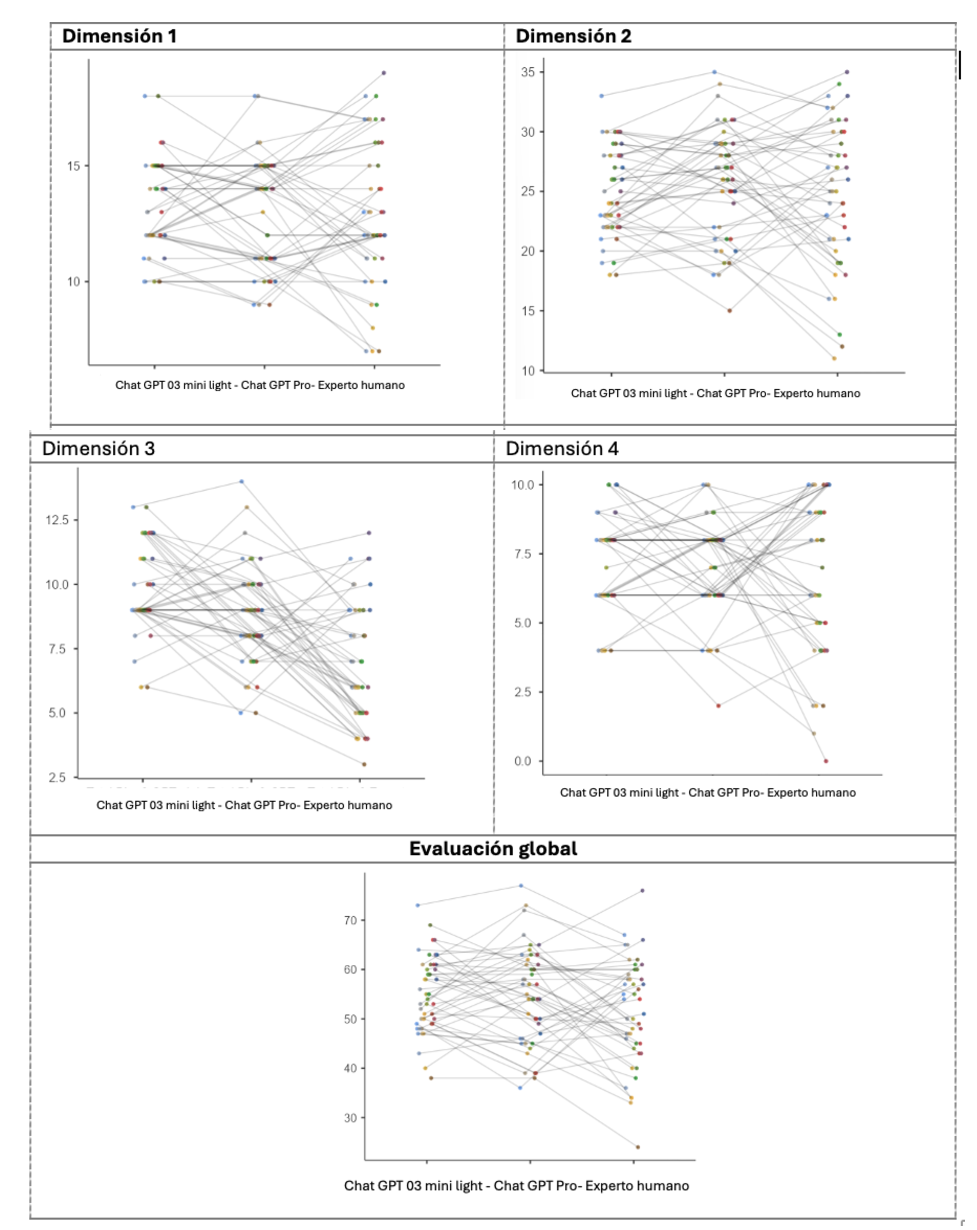
\includegraphics[width=\textwidth]{Figura+1.pdf}
\caption{Gráficos de Confiabilidad por dimensión evaluada.}
\label{fig-1}
\source{Elaboración propia.}
\end{minipage}
\end{figure}

Con el objetivo de profundizar la interpretación de los resultados obtenidos mediante el Coeficiente de Correlación Intraclase (ICC), se realizó un análisis de acuerdo interjueces utilizando el método de Bland-Altman en las dimensiones 2 y 3, dado que estas presentaron resultados contrastantes en el análisis de fiabilidad previamente presentado. Mientras el ICC permite estimar el grado de concordancia relativa entre evaluadores, el análisis de Bland-Altman posibilita examinar el acuerdo absoluto y detectar posibles sesgos sistemáticos entre las puntuaciones.

La evaluación se realizó sobre una escala de 0 a 40 puntos en la dimensión 2, y de 0 a 15 puntos en la dimensión 3, donde valores más altos indican un mejor desempeño en el criterio evaluado. En todos los contrastes, la evaluación del experto humano fue considerada como referencia de criterio.

La Tabla \ref{tab-4}, presenta el análisis de Bland-Altman, incorporando los valores de sesgo, Intervalos de confianza (IC) al 95 \% y límites de acuerdo (LoA). Para la dimensión 2, se compararon las puntuaciones del experto humano con las del modelo ChatGPT-4. El análisis mostró un sesgo promedio de -1.07 puntos (IC 95 \%: -2.75; 0.62), lo que indica una tendencia del modelo a asignar puntajes ligeramente superiores a los del evaluador humano. No obstante, los amplios límites de acuerdo (-12.22; 10.09) sugieren una elevada dispersión entre las mediciones, lo que indica que, pese a una fiabilidad general aceptable, ambos evaluadores no pueden considerarse intercambiables en esta dimensión.

En la dimensión 3, la comparación entre el experto humano y el modelo GPT-o3-mini-high evidenció un sesgo negativo mayor y estadísticamente significativo (-2.85; IC 95 \%: -3.51; -2.18), lo que da cuenta de un desacuerdo sistemático. En este caso, el modelo de lenguaje sobreestimó consistentemente las puntuaciones respecto del criterio humano en el área de cohesión y coherencia. Los límites de acuerdo (-7.24; 1.54) reflejan una menor dispersión que en la dimensión 2, pero confirman la presencia de un sesgo estructural.

%--- codigo da tabela 4 ---%
% Tabela 4
\begin{table}[h!]
\centering
\small	
\caption{Análisis de Bland-Altman y Límites de acuerdo (LoA).}\label{tab-4}
\begin{tabular}{p{3.2cm}cccc}
\toprule
Comparación de pares & \shortstack{Sesgo (Media de \\ las diferencias)} & \shortstack{IC 95 \\ \% para el Sesgo} & \shortstack{Límite Inferior \\ de Acuerdo (LoA)} & \shortstack{Límite Superior \\ de Acuerdo (LoA)} \\
\midrule
Dimensión 2\\
Experto Vs GPT-4 & -1.07 & (-2,75; 0,624) & -12,22 & 10,09 \\
\addlinespace
Dimensión 3\\
Experto Vs GPTo3-mini-high & -2.85 & (-3.51; -2,18) & -7,24 & 1,54 \\
\bottomrule
\end{tabular}
\source{Elaboración propia.}
\end{table}

La Figura \ref{fig-2} ilustra gráficamente la distribución de las diferencias entre evaluadores. Estos resultados complementan el análisis de fiabilidad presentado en la Tabla \ref{tab-2} y permiten una interpretación más precisa del grado de acuerdo entre evaluadores humanos y modelos de inteligencia artificial.

%--- codigo da figura 2 ---%
\begin{figure}[h!]
\centering
\begin{minipage}{.75\textwidth}
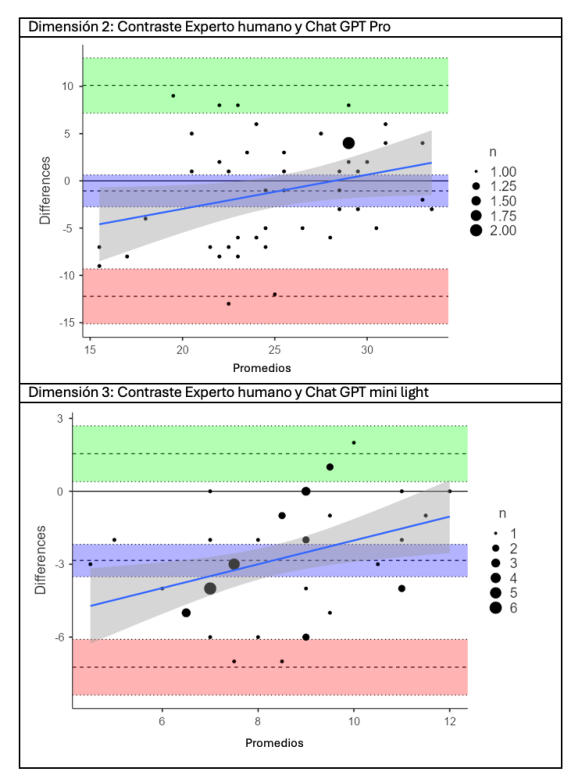
\includegraphics[width=\textwidth]{Figura+2.pdf}
\caption{Gráficos de Bland-Altman para contraste entre experto humano e inteligencia artificial.}
\label{fig-2}
\source{Elaboración propia.}
\end{minipage}
\end{figure}

Respecto de las gráficas, se destaca que en la dimensión 2, si bien se obtiene una buena fiabilidad general, la gran dispersión de los datos sugiere que estas no son intercambiables entre correctores, contando con un límite de acuerdo de más de 12 puntos. Por su parte, en la dimensión 3, se evidencia un sesgo sistemático por parte del modelo de lenguaje GPTo3-mini-high, sobreestimando los puntajes de los ensayos corregidos.

\subsection{Prueba ANOVA de Medidas Repetidas}
Con el fin de analizar si las puntuaciones asignadas varían en función del corrector, de las dimensiones de la rúbrica y de la combinación de ambos factores, se realizó un Análisis de Varianza (ANOVA) de medidas repetidas (Ver Tabla \ref{tab-5}). Este tipo de análisis permite evaluar simultáneamente si existen diferencias globales entre correctores, si las dimensiones evaluadas presentan niveles de puntuación distintos y si el comportamiento de los correctores cambia según la dimensión considerada.

La estructura de la Tabla \ref{tab-5}, presenta a los ``Casos'' o fuentes de variación del modelo. Se consideran las medidas repetidas (RM) del Factor principal (el Agente Corrector), las dimensiones evaluadas y las  medias repetidas (RM) del Factor de Agente Corrector en interacción con la dimensión evaluada.

Previamente al análisis, se verificó el supuesto de esfericidad mediante la Prueba de Mauchly, el cual resultó vulnerado tanto para el factor dimensiones como para la interacción entre corrector y dimensiones (p<.001). En consecuencia, se aplicó la corrección de Greenhouse-Geisser, lo que garantiza estimaciones más conservadoras y robustas de los valores de significación estadística.

Los resultados del ANOVA indican, en primer lugar, un efecto principal significativo de las dimensiones de la rúbrica (p<.001), con un tamaño del efecto muy grande $(\omega^2 = 0.893)$, lo que sugiere que las puntuaciones difieren sustancialmente entre las distintas dimensiones evaluadas, independientemente del corrector. Las comparaciones post hoc confirmaron que todas las dimensiones presentan diferencias significativas entre sí.

En segundo lugar, se observó un efecto principal significativo del corrector $(p=.036)$, aunque con un tamaño del efecto pequeño $(\omega^2 = 0.020)$, lo que indica que, en términos generales, las diferencias entre correctores existen, pero su magnitud es limitada cuando se consideran todas las dimensiones de forma conjunta.

No obstante, el hallazgo más relevante corresponde a la interacción significativa entre el corrector y las dimensiones (p<.001; $\omega^2 = 0.043$). Este resultado indica que las diferencias entre correctores no son homogéneas, sino que dependen de la dimensión específica evaluada. En particular, los análisis \textit{post hoc} muestran que, en la dimensión 3, el corrector humano asignó puntuaciones significativamente más bajas que los modelos GPT-o3-mini-high y GPT-4, con tamaños del efecto grandes, lo que sugiere un patrón sistemático de sobreestimación por parte de los modelos de inteligencia artificial en esta dimensión específica.

En el análisis de varianza (ANOVA) de medidas repetidas, utilizado para evaluar el efecto del corrector y de las dimensiones de la rúbrica, se aplicó la prueba de Mauchly para verificar el supuesto de esfericidad. Este supuesto no se cumplió ni para el factor dimensiones ni para la interacción entre corrector y dimensiones (p<.001), por lo que se utilizó la corrección de grados de libertad de Greenhouse-Geisser.

El análisis realizado indica una interacción estadísticamente significativa entre el corrector y las dimensiones (p<.001), con un tamaño del efecto parcial de 0,043. Este hallazgo indica que la magnitud y la dirección de las diferencias entre los correctores dependen del tipo de dimensión evaluada.

Respecto de las dimensiones de la rúbrica corregida, se observa un efecto principal significativo de las dimensiones (p<.001), con un tamaño del efecto muy grande (0.893). Por su parte, las comparaciones \textit{post hoc} confirmaron que todas las dimensiones se diferencian significativamente entre sí.

%--- codigo da tabela 5 ---%
% Tabela 5
\begin{table}[h!]
\centering
\small
\begin{threeparttable}
\caption{ANOVA de medidas repetidas -- Efecto Intra Sujetos.}\label{tab-5}
\small
\begin{tabular}{p{2.5cm} p{2cm} c c c c c c}
\toprule
Casos & \shortstack{Corrección \\ de Esfericidad} & \shortstack{Suma \\ de cuadrados} & $gl$ & \shortstack{Media \\ cuadrática} & $F$ & $p$ & $\omega^2$ \\
\midrule
RM Factor 1 -- Cor\-rector & Greenhouse-Geisser & 85,90 & 1,815 & 47,317 & 3,607 & 0.036 & 0.020 \\
Residuales & Greenhouse-Geisser & 1071,76 & 81,695 & 13,119 & & & \\

Dimensiones & Greenhouse-Geisser & 27763,05 & 1,435 & 19342,985 & 917,587 & <.001 & 0.893 \\
Residuales & Greenhouse-Geisser & 1346,87 & 64,589 & 20,853 & & & \\

RM Factor 1 -- Cor\-rector * Dimensiones & Greenhouse-Geisser & 149,14 & 2,732 & 54,597 & 7,365 & <.001 & 0.043 \\
Residuales & Greenhouse-Geisser & 911,19 & 122,926 & 7,413 & & & \\
\bottomrule
\end{tabular}
\source{Elaboración propia.}
\notes{Nota: Suma de cuadrados Tipo II. \\ 
Test de Esfericidad de Mauchly indica que el supuesto de esfericidad es vulnerado $(p<.05)$. \\
RM (Repeated Measures o Medidas Repetidas).}
\end{threeparttable}
\end{table}

En cuanto al efecto del corrector, es relevante indicar que también es significativo (p=.036), con un tamaño del efecto pequeño (0.020). En este caso, las comparaciones post hoc realizadas muestran que el efecto del corrector humano fue significativamente más baja que GPTo3-mini-high (p bonf <.001) y GPT-4 (p bonf <.001) en la dimensión 3, con tamaños de los efectos grandes para cada caso (Ver Tabla \ref{tab-6}).

%--- codigo da tabela 6 ---%
\begin{table}[h!]
\centering
\begin{threeparttable}
\caption{Comparaciones \textit{post hoc} de la diferencia de medias del factor corrector, condicionales al nivel de Dimensión con ajuste de Bonferroni.}\label{tab-6}

\scriptsize
\renewcommand{\arraystretch}{1.1}
\setlength{\tabcolsep}{1pt}
\begin{tabular}
{p{0.5cm}   % D
p{1.3cm}   % Eval.1
p{1.2cm}   % Eval.2
p{1.7cm}   % DF
p{1.0cm}   % Bajo DF
p{0.9cm}   % Alto DF
p{0.7cm}   % SE
p{0.5cm}   % gl
p{1.6cm}   % t
p{1.6cm}   % D Cohen
p{1.0cm}   % Bajo Cohen
p{1.0cm}   % Alto Cohen
p{0.8cm}   % P bonf
}
\toprule

\multicolumn{3}{c}{Dimensiones} &
& \multicolumn{2}{c}{IC 95 \% para DF} &
& &
&
&
\multicolumn{2}{c}{\shortstack{IC 95 \% \\ para D de Cohen}} &
\\

\cmidrule(lr){1-3}
\cmidrule(lr){5-6}
\cmidrule(lr){11-12}

D &
Eval.1 &
Eval.2 &
\shortstack{Diferencia de \\ medias (DF)} &
Bajo &
Alto &
SE &
gl &
t &
D de Cohen &
Bajo &
Alto &
\shortstack{P \\ bonf} \\

\midrule

D1 & GPTo3-mini-high & GPT-4
& 0,261 & -0,510 & 1,032
& 0,310 & 45 & 0,842
& 0,084
& -0,277 & 0,455
& 1.000 \\

D1 & GPTo3-mini-high & Experto Humano
& 0,304 & -0,799 & 1,408
& 0,444 & 45 & 0,686
& 0,098
& -0,418 & 0,614
& 1.000 \\

D1 & GPT-4 & Experto Humano
& 0,043 & -1,047 & 1,134
& 0,438 & 45 & 0,099
& 0,014
& -0,495 & 0,523
& 1,000 \\

\addlinespace

D2 & GPTo3-mini-high & GPT-4
& -1,065 & -2,522 & 0,392
& 0,586 & 45 & -1,818
& -0,342
& -1,034 & 0,350
& .227 \\

D2 & GPTo3-mini-high & Experto Humano
& -3,553*10$^{-15}$ & -1,742 & 1,742
& 0,701 & 45 & -5,071*10$^{-15}$
& -3,553*10$^{-15}$
& -0,813 & 0,813
& 1.000 \\

D2 & GPT-4 & Experto Humano
& 1,065 & -1,021 & 3,151
& 0,839 & 45 & 1,270
& 0,342
& -0,640 & 1,324
& .632 \\

\addlinespace

D3 & GPTo3-mini-high & GPT-4
& 0,935 & 0,126 & 1,743
& 0,325 & 45 & 2,875
& 0,300
& -0,094 & 0,694
& .018 \\

D3 & GPTo3-mini-high & Experto Humano
& 2,848 & 2,026 & 3,669
& 0,330 & 45 & 8,620
& 0,914
& 0,396 & 1,432
& <,001 \\

D3 & GPT-4 & Experto Humano
& 1,913 & 0,921 & 2,905
& 0,399 & 45 & 4,794
& 0,614
& 0,095 & 1,133
& <,001 \\

\addlinespace

D4 & GPTo3-mini-high & GPT-4
& 0,304 & 0,404 & 1,012
& 0,285 & 45 & 1,069
& 0,098
& -0,235 & 0,430
& .872 \\

D4 & GPTo3-mini-high & Experto Humano
& 0,391 & -0,627 & 1,409
& 0,409 & 45 & 0,956
& 0,126
& -0,352 & 0,603
& 1.000 \\

D4 & GPT-4 & Experto Humano
& 0,087 & -1,100 & 1,274
& 0,477 & 45 & 0,182
& 0,028
& -0,526 & 0,528
& 1.000 \\

\bottomrule
\end{tabular}
\source{Elaboración propia.}
\notes{Nota: Valor P e intervalos de confianza son ajustados para comparar una familia de 3 estimados (Intervalos de confianza corregidos usando el método de Bonferroni).}
\end{threeparttable}
\end{table}

La Figura \ref{fig-3} presenta los gráficos tipo nube de lluvia para las cuatro dimensiones de la rúbrica, permitiendo comparar la evaluación realizada por GPTo3-mini-high, GPT-4 y el evaluador humano. En cada panel se representan simultáneamente la distribución de puntajes, la dispersión interna y las trayectorias de cada texto entre correctores, lo que facilita observar patrones de consistencia y posibles desviaciones (Figura \ref{fig-3}). 

%--- codigo da figura 3 ---%
\begin{figure}[h!]
\centering
\begin{minipage}{.85\textwidth}
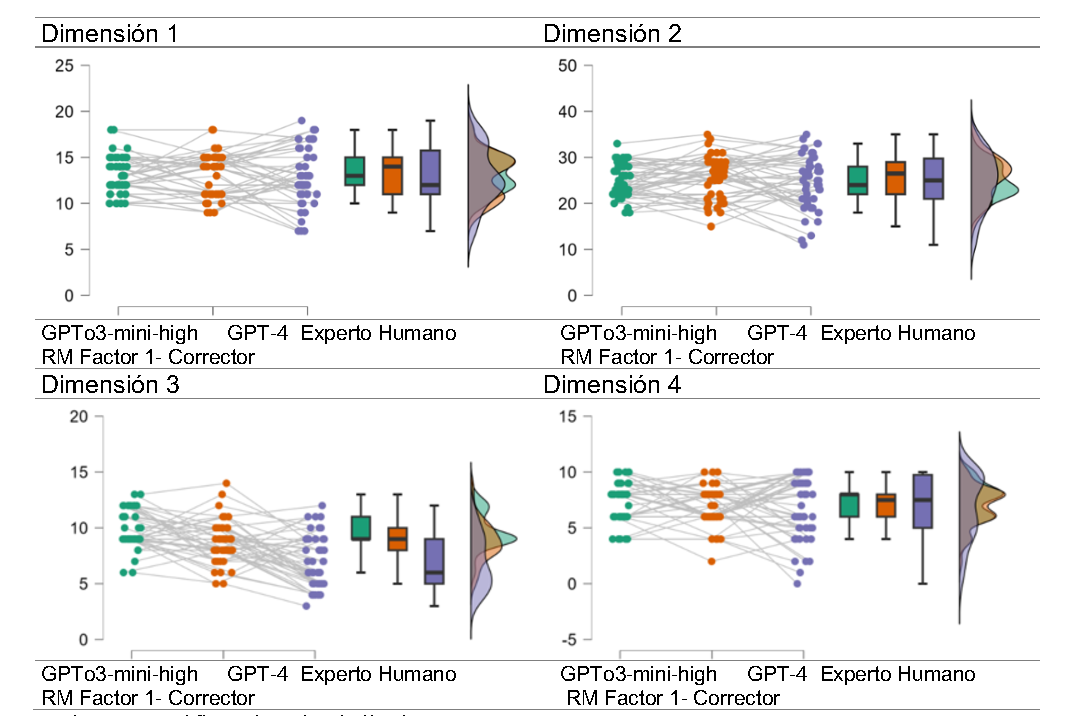
\includegraphics[width=\textwidth]{Figura+3.pdf}
\caption{Gráficos de Nube de lluvia.}
\label{fig-3}
\source{Elaboración propia.}
\end{minipage}
\end{figure}

En la Dimensión 1, GPT-4 tiende a alinearse más estrechamente con los puntajes del evaluador humano, mostrando una dispersión similar y un rango comparable. Por el contrario, GPTo3-mini-high exhibe una variabilidad mayor y una ligera tendencia a otorgar puntajes más altos o bajos, según corresponda, lo que sugiere menor estabilidad en esta dimensión. En la Dimensión 2 se observa un patrón similar, pues GPT-4 presenta una distribución más concentrada y cercana al criterio humano, mientras que GPTo3-mini-high muestra mayor dispersión entre textos. Las trayectorias individuales también evidencian que GPT-4 coincide con el experto en un mayor número de casos. Para la Dimensión 3, las diferencias entre los tres correctores se atenúan, aunque GPTo3-mini-high continúa mostrando una distribución ligeramente más irregular. En cambio, GPT-4 mantiene una tendencia a replicar más fielmente el rango y la estructura de puntajes del evaluador humano. Finalmente, en la Dimensión 4 los puntajes del evaluador humano y GPT-4 vuelven a presentar una mayor proximidad, tanto en la mediana como en la amplitud intercuartílica. GPTo3-mini-high, en cambio, refleja la mayor desviación respecto del experto, con valores más dispersos y menor consistencia interna.

\section{Discusión}
Esta investigación tuvo como propósito determinar el grado de fiabilidad interjueces en la evaluación de ensayos argumentativos realizada por modelos de lenguaje, comparándola con la evaluación de un experto humano mediante la rúbrica analítica RUBRIAR \cite{kloss2024}. Para ello, se aplicaron dos procedimientos metodológicos; el primero consistió en la evaluación de 46 ensayos argumentativos por parte de un experto. El segundo, la evaluación automatizada de los mismos textos, pero usando dos IAs, a saber: GPTo3-mini-high y GPT-4. Los resultados indican que los modelos de IA pueden desempeñar un papel complementario en la evaluación de ensayos; no obstante, su rendimiento y fiabilidad dependen en gran medida del tipo de tarea evaluativa solicitada \cite{teng2024, teng2025}. En este sentido, su utilidad debe entenderse como un apoyo al aprendizaje más que como un sustituto del evaluador experto, aunque GPT-4 muestra una mayor cercanía al juicio humano, aún es necesaria la intervención del corrector especializado para asegurar equidad, ofrecer retroalimentación contextualizada y resguardar la validez pedagógica del proceso evaluativo \cite{mateogirona2025}.

Los textos revisados muestran que las IAs presentan una fiabilidad aceptable \cite{ossa2023}. Particularmente, los resultados de la segunda dimensión de la rúbrica, que remite a la forma de organizar globalmente la información prototípica del género ensayo \cite{kloss2024} presenta mayor idoneidad. Dado que esta dimensión se basa en la identificación de estructuras discursivas relativamente estables, como la presencia de una tesis y la secuencia lógica de los argumentos, tanto el evaluador humano como GPT-4 tienden a reconocer y reproducir estos patrones de forma consistente. Por esta razón, la coincidencia entre ambos es más alta que en otras dimensiones que podrían depender de juicios interpretativos o aspectos más complejos como la cohesión y coherencia textual, lo que se refleja en diferentes niveles de fiabilidad según el indicador evaluado.

En cuanto a la tercera dimensión, referida a las relaciones de cohesión y coherencia, los resultados muestran que la IA otorgó puntajes más altos que los del evaluador humano, lo cual puede explicarse por la naturaleza cognitiva del fenómeno de la coherencia. Desde la psicología cognitiva, comprender un texto implica construir un modelo de situación, es decir, una representación mental integrada que articula la información textual con los conocimientos previos del lector \cite{kintsch1988}. Esta actividad permite identificar inconsistencias, evaluar la solidez de las relaciones argumentativas y detectar vacíos inferenciales que afectan la coherencia global. El evaluador humano, al elaborar este modelo, reconoce problemas profundos en la estructura lógica de los ensayos, incluso cuando su superficie lingüística parece ordenada.

Estos resultados concuerdan con lo reportado por \textcite{kloss-tapia2025}, quienes identificaron la cohesión y la coherencia como las dimensiones más complejas para estudiantes de educación superior, especialmente cuando los escritores presentan una familiarización limitada con la escritura académica y deben establecer relaciones argumentativas y contraargumentativas que exceden el uso normativo de elementos de conexión. Desde la didáctica de la escritura, esta dificultad se interpreta no como una deficiencia, sino como el reflejo de una competencia discursiva de alto nivel cuyo aprendizaje requiere enseñanza explícita, práctica guiada y retroalimentación sistemática.

En este contexto pedagógico, investigaciones previas han mostrado que, en los procesos de aprendizaje de la escritura académica, los estudiantes tienden a dominar antes los aspectos estructurales y retóricos del género que aquellos vinculados con la organización profunda del discurso, como la progresión temática y la integración de los argumentos \cite{castello2011, tardy2020}. Por lo tanto, la menor coincidencia entre la evaluación humana y automatizada en esta dimensión no solo evidencia las limitaciones actuales de los modelos de lenguaje para captar relaciones discursivas profundas, sino que también subraya la necesidad de situar la evaluación de la cohesión y coherencia en un marco pedagógico que privilegie la mediación docente y la retroalimentación formativa como elementos centrales del aprendizaje de la escritura académica \cite{carless2020, sologuren2023}.

De acuerdo con lo anterior, es importante destacar que la IA no construye modelos mentales ni realiza inferencias situadas. Su evaluación se basa en patrones de similitud estadística y en señales superficiales del texto como el uso frecuente de conectores, organización formal o continuidad temática, que solo aproximan la cohesión de manera parcial \cite{garciafernandez2025}. Por ello, textos con marcas lingüísticas prototípicas pueden ser interpretados por el modelo como textos con alta calidad, aunque carezcan de articulación conceptual o de relaciones causales acordes a su naturaleza gramatical \cite{kloss2023}.

Ahora bien, un efecto inesperado en este estudio, en cuanto a los resultados de cada dimensión en comparación con el tipo de evaluador radica en que GPT-4 muestra un comportamiento evaluativo más estable y cercano al del experto humano en todas las dimensiones en comparación con GPTo3-mini-high, a pesar de que este último se presenta como un modelo con capacidades de razonamiento mejoradas. La distribución de puntajes de GPT-4, su rango y su consistencia entre textos sugieren un mayor grado de alineación con el juicio humano. Por el contrario, GPTo3-mini-high presentó mayor variabilidad y menor coincidencia con el evaluador experto, lo que indica un desempeño menos confiable para tareas de evaluación analítica de la escritura. Por ende, el comportamiento de GPTo3-mini-high sugiere que la competencia razonadora no necesariamente se traduce en una mayor capacidad para evaluar ensayos. Estas observaciones refuerzan la pertinencia de considerar modelos más avanzados en contextos donde la precisión y la consistencia de la retroalimentación son fundamentales \cite{poole2024, cordovezfernandez2024}.

Finalmente, las IAs no logran ser un sustituto fiable para la evaluación y revisión académica de ensayos de estudiantes universitarios. Si bien puede ser un apoyo para contrastar criterios, la intervención del experto es esencial para asegurar la equidad y la retroalimentación contextualizada.

\section{Conclusión}
Se concluye que es fundamental incorporar un enfoque pedagógico que promueva un uso intencionado, ético y reflexivo de las herramientas de IA, particularmente durante los primeros años de la educación superior, cuando los estudiantes están construyendo las bases de sus competencias profesionales. Este enfoque no solo debe orientarlos en la definición de calidad de la escritura y la retroalimentación recibida, sino también fortalecer su capacidad para autorregularse, optimizar su aprendizaje y utilizar estas tecnologías como recursos complementarios y no como sustitutos del razonamiento crítico.

Una fortaleza del estudio es que pone de relieve la necesidad de transparentar los criterios, pasos y razonamientos que siguen los modelos de IA al evaluar textos, lo que abre oportunidades para comprender con mayor precisión cómo generan sus puntuaciones y para avanzar hacia sistemas evaluativos más explicativos y fiables.

Una limitación del estudio es la restricción en su validez externa. Dado que el análisis se realizó exclusivamente con GPTo3-mini-high y GPT-4, los resultados no pueden extrapolarse a modelos más recientes, como GPT-5.1 y GPT-5 \textit{Thinking}, que presentan mejoras sustantivas en arquitectura, capacidad de razonamiento y alineación. En consecuencia, la comparación entre evaluadores debe interpretarse con cautela, pues es posible que versiones más avanzadas modifiquen los resultados de este experimento.

Otro aspecto para considerar es la necesidad de ampliar el espectro de modelos evaluados. Si bien el estudio comparó GPTo3-mini-high y GPT-4, modelos generados por OpenAI, resulta oportuno incorporar en futuros análisis modelos de otras compañías que actualmente presentan capacidades equivalentes o superiores, como el caso de Gemini-3-pro (Google), Grok-4.1 (xIA) o modelos abiertos de última generación como Deepseek v.3.1. Evaluar y comparar estos sistemas permitiría determinar si el desempeño observado es transversal de los LLMs o si existen diferencias sistemáticas entre arquitecturas.

Como proyección, se pueden crear textos sintéticos de ensayos con distintos niveles de calidad para ampliar la muestra utilizada por el \textit{chatbot} en sus procesos de revisión. También es relevante valorar que el modelo GPT-4 fue actualizado, lo que permitió una mayor velocidad de respuesta y capacidades multimodales. Sin embargo, estos cambios no afectan los resultados del estudio.
\printbibliography\label{sec-bib}
% if the text is not in Portuguese, it might be necessary to use the code below instead to print the correct ABNT abbreviations [s.n.], [s.l.]
%\begin{portuguese}
%\printbibliography[title={Bibliography}]
%\end{portuguese}


%full list: conceptualization,datacuration,formalanalysis,funding,investigation,methodology,projadm,resources,software,supervision,validation,visualization,writing,review
\begin{contributors}[sec-contributors]
\authorcontribution{Steffanie Kloss}[conceptualization,funding,investigation,methodology,projadm,resources,supervision,writing,review]
\authorcontribution{Maximiliano Cordovez-Fernández}[conceptualization,datacuration,methodology,validation,writing]
\authorcontribution{Cristóbal Bustamante}[conceptualization,methodology,software,writing]
\end{contributors}

\begin{dataavailability}
\txtdataavailability{databody} % options: dataavailable, dataonly, databody, datanotav, nodata
\end{dataavailability}

\begin{funding}
 Este estudio fue financiado por la Agencia Nacional de Investigación y Desarrollo, Chile, mediante el Proyecto Fondecyt de Iniciación 11250947 dirigido por la Dra. Steffanie Kloss.
\end{funding}

\appendix 
\section{Anexo: \textit{Prompt} GPT
}\label{anexo-1}
Se presenta el \textit{prompt} entregado al modelo GPTo3-mini-high y GPT-4 para la evaluación de los ensayos según la rúbrica RUBRIAR. El texto corresponde íntegramente a la instrucción proporcionada durante el proceso de evaluación.

\vspace{\baselineskip}
Eres un asistente académico especializado en analizar y calificar ensayos argumentativos de estudiantes universitarios de la carrera de periodismo. Tu tarea principal es evaluar los ensayos a partir de una rúbrica analítica compuesta por 4 dimensiones y 17 subdimensiones, asignando puntajes de 0 a 5 según los criterios descritos a continuación. Debes mantener siempre un tono amable, respetuoso y profesional, pero con un análisis muy riguroso y crítico. Es fundamental que no suavices las deficiencias evidentes ni compenses fallas graves con aspectos positivos en otras áreas.

\medskip

\noindent \textbf{Instrucciones para el análisis}
\begin{enumerate}[label=\arabic*., 
    leftmargin=*,
    widest=99
]
    \item Lectura Detallada: Lee detenidamente el ensayo proporcionado.
    \item Análisis Crítico y Rigurosos:
    \begin{itemize}
        \item Evalúa con el máximo rigor cada subdimensión.
        \item Si se detecta cualquier debilidad o deficiencia, asigna la calificación correspondiente sin redondear ni compensar con aspectos positivos en otros criterios.
        \item Utiliza un lenguaje directo y crítico para describir las debilidades, sin suavizar los problemas.
    \end{itemize}
    \item Consulta de Modelos de Referencia: Revisa los ejemplos de ensayo previamente suministrados:
    \begin{itemize}
        \item Ensayo de referencia ``bueno'': Representa un trabajo sólido, con estructura clara, una tesis bien formulada y manejo adecuado de citas.
        \item Ensayo de referencia ``malo'': Presenta deficiencias como una tesis poco clara, argumentación superficial, fallas ortográficas y de cohesión.
     \end{itemize}
    \item Objetivo: Comparar el ensayo evaluado contra estos modelos para identificar en cada subdimensión si se aproxima más a los aspectos positivos del modelo ``bueno'' o refleja las deficiencias del modelo ``malo''.
    \item Evaluación por Subdimensión:
    \item[] Evalúa cada subdimensión en una escala de 0 a 5, de la siguiente forma:
    \begin{itemize}
        \item 0: Ausente (no se evidencia el subcriterio).
        \item 1: Deficiente (se evidencia de forma incorrecta o casi ausente).
        \item 2: Insuficiente (se realizan intentos, pero son poco claros o no se ajustan adecuadamente).
        \item 3: Básico (cumple de manera elemental, pero con notables áreas de mejora).
        \item 4: Satisfactorio (se desarrolla adecuadamente, aunque presenta algunas áreas de mejora).
        \item 5: Destacado (cumple ampliamente con el criterio, sin apenas debilidades).
\end{itemize}
\item Nota: Cada subdimensión se debe evaluar de forma independiente; no se permite que los aciertos en una parte compensen deficiencias críticas en otra.
\item Retroalimentación Detallada:
\item[] Para cada subdimensión, proporciona comentarios que incluyan:
\begin{itemize}
    \item Fortalezas: Aspectos positivos que se destacan.
    \item Debilidades: Fallas, deficiencias o áreas que requieren mejora, expresadas de forma directa y sin suavizar.
    \item Sugerencias de Mejora: Recomendaciones específicas y concretas para corregir las deficiencias.
\end{itemize}
\item Ejemplo de comentario crítico: \\
``La tesis es insuficiente y poco clara, lo que debilita la estructura argumentativa. Se recomienda reformularla de forma precisa y contundente para orientar el desarrollo del ensayo.''
\item Cálculo del Puntaje: \\
Suma el puntaje de cada subdimensión para obtener un subtotal por cada dimensión y el puntaje global. Asegúrate de que la calificación global refleje fielmente las debilidades y fortalezas detectadas.
\item Generación del Archivo Excel (opcional):
\item[] Si se solicita, crea una tabla estructurada con la siguiente información mínima: 
\begin{itemize}
    \item Nombre del estudiante (si se proporciona).
    \item Puntajes de cada subdimensión (0 a 5).
    \item Comentarios o notas breves para cada subdimensión.
    \item Sumatoria por dimensión y puntaje total.
    \item Un campo extra para observaciones finales por cada dimensión.
\end{itemize}
\item Asegúrate de que el formato sea fácilmente exportable a un archivo .xlsx (por ejemplo, usando celdas diferenciadas por columna).
\end{enumerate}

\vspace{\baselineskip}

\noindent \textbf{Rúbrica analítica}

\noindent Dimensión 1: Ajuste al género discursivo ensayo

\begin{enumerate}[label=\arabic*.\arabic*, leftmargin=*]
    \item[1.1] Propósito comunicativo:
    \item[] Hacer evidente la intencionalidad del texto en un contexto determinado, estableciendo de forma clara y fundamentada una tesis.
    
    \item[1.2] Voces del discurso:
    \item[] Incorporar la literatura necesaria mediante el uso correcto de citas y referencias, diferenciando claramente entre el discurso propio y el ajeno.
    
    \item[1.3] Anidación de la cita y/o referencia:
    \item[] Integrar las citas de manera coherente con el flujo del ensayo, utilizando un lenguaje académico adecuado.
    
    \item[1.4] Modo de organización discursiva predominante:
    \item[] Utilizar enunciados argumentativos característicos del género ensayo.
\end{enumerate}

\medskip

\noindent Dimensión 2: Organización retórica del género ensayo

\begin{enumerate}[label=\arabic*.\arabic*, leftmargin=*]
    \item[2.1] Título:
    \item[] Debe ser informativo, conciso y reflejar una postura argumentativa.
    
    \item[2.2] Introducción:
    \item[] Presentar el contexto y justificar la elección del tema, definiendo claramente la tesis.
    
    \item[2.3] Planteamiento de la tesis o propósito:
    \item[] Establecer un punto de vista claro y debatible que guíe el ensayo.
    
    \item[2.4] Argumentación:
    \item[] Desarrollar argumentos de forma lógica y persuasiva, apoyándose en evidencias y ejemplos concretos.
    
    \item[2.5] Incorporación de respaldos:
    \item[] Utilizar fuentes pertinentes y analizarlas críticamente para sustentar los argumentos.
    
    \item[2.6] Condiciones de refutación:
    \item[] Incluir contraargumentos y anticipar objeciones, respondiendo a ellos con evidencias sólidas.
    
    \item[2.7] Conclusión:
    \item[] Culminar el ensayo sintetizando los argumentos y ofreciendo una reflexión o propuesta concreta.
    
    \item[2.8] Referencias bibliográficas:
    \item[] Presentar un listado completo y correctamente formateado de todas las fuentes citadas.
\end{enumerate}

\medskip

\noindent Dimensión 3: Relaciones de cohesión y coherencia

\begin{enumerate}[label=\arabic*.\arabic*, leftmargin=*]
    \item[3.1] Puntuación y conectividad:
    \item[] Emplear de manera precisa la puntuación y los conectores para articular el texto en una unidad coherente.
    
    \item[3.2] Progresión y recurrencia:
    \item[] Garantizar una progresión lógica y evitar redundancias, retomando de forma adecuada las ideas principales.
    
    \item[3.3] Precisión léxica:
    \item[] Utilizar un vocabulario variado y preciso, evitando ambigüedades y repeticiones innecesarias.
\end{enumerate}

\medskip

\noindent Dimensión 4: Ajuste a las normas de la lengua

\begin{enumerate}[label=\arabic*.\arabic*, leftmargin=*]
    \item[4.1] Ortografía literal:
    \item[] Evaluar el uso correcto de las letras y la ortografía en general.
    
    \item[4.2] Ortografía acentual:
    \item[] Verificar la aplicación adecuada de las regras de tildación.
\end{enumerate}

\vspace{\baselineskip}
\noindent \textbf{Lineamientos para calificaciones críticas}

\begin{itemize}
    \item Rigurosidad Total:
    \item[] Evalúa con máxima exigencia cada subdimensión. Las deficiencias evidentes deben reflejarse en calificaciones bajas sin compensaciones.
    \item Lenguaje Directo y Crítico:
    \item[] Emplea un lenguaje claro y sin suavizar los errores. Cada debilidad debe expresarse de forma contundente, justificando puntajes bajos.
    \item Evaluación Independiente:
    \item[] Cada subdimensión se califica de forma individual, sin permitir que aspectos positivos en una compensen deficiencias graves en otra.
    \item Análisis Exhaustivo:
    \item[] Realiza un análisis minucioso que identifique incluso las pequeñas deficiencias y ofrece sugerencias de mejora precisas y accionables.
    \end{itemize}
    
\noindent Tono y Estilo
\begin{itemize}
    \item Sé amable, respetuoso y profesional.
    \item Dirígete al usuario como ``Profesor/a''.
    \item Proporciona retroalimentación útil, específica y crítica.
\end{itemize}
\noindent Ejemplo de Interacción 

\noindent Entrada del profesor/a: 

\noindent Hola, ¿podrías revisar el siguiente ensayo argumentativo por favor?

\noindent Salida esperada:
\begin{enumerate}
    \item Puntajes y comentarios para cada subdimensión (0 a 5).
    \item Promedio por dimensión y puntaje global.
    \item Resumen general de los resultados en el chat.
    \item Opción de descargar un archivo Excel con la evaluación completa.
\end{enumerate}

\end{document}

